\documentclass[a5paper, oldfontcommands, hidelinks]{ufsc-thesis}  % escolha o tamanho do papel aqui

\usepackage{cmap}
\usepackage[utf8]{inputenc}
\usepackage[T1]{fontenc}

\usepackage{textcomp}

%---- Bibliography packages ----%

\usepackage[style=numeric, sorting=none]{biblatex}
\DeclareNameAlias{author}{last-first}
\addbibresource{bibliography.bib}

%---- Units Packages ----%

\usepackage{siunitx}

%---- Drawing Packages ----%

\usepackage{tikz}
\usepackage{circuitikz}
\usepackage{pgfplots}
\pgfplotsset{compat=1.5}

\usetikzlibrary{positioning}

\usepackage{tikz}
\usetikzlibrary{shapes,arrows}

\tikzstyle{decision} = [diamond, draw, fill=black!20, 
    text width=4.5em, text badly centered, node distance=3cm, inner sep=0pt]
\tikzstyle{process} = [rectangle, draw, fill=black!20, 
    text width=5em, text centered, rounded corners, minimum height=4em]
\tikzstyle{line} = [draw, -latex']


%---- Lists Packages ----%
\usepackage[acronym, automake, nomain, nonumberlist]{glossaries-extra}

% Preâmbulo
\titulo{}
\autor{Bruno Vale Barbosa Eiterer}
\data{\today}
\instituicao{Universidade Federal de Santa Catarina}
\local{Florianópolis, SC}
\tipotrabalho{}
\orientador{Prof. Eduardo Augusto Bezerra, Ph.D.}
\coorientador{Leonardo Kessler Slongo, Ms.C.}
\programa{Engenharia Elétrica}
\preambulo{}
\centro{}
\assuntos{}

\setabbreviationstyle[acronym]{long-short}
\makeglossaries
\loadglsentries[\acronymtype]{glossary}

\begin{document}
% Inicia parte pré-textual do documento capa, folha de rosto, folha de
% aprovação, aprovação, resumo, lista de tabelas, lista de figuras, etc.
\pretextual%
\imprimircapa%!
\imprimirfolhaderosto*%
\clearpage
\imprimirfichacatalografica%
%\tableofcontents%
\textual%

\glsaddall 
\printglossary[type=\acronymtype, title = Lista de Abreviaturas e Siglas]

\begin{refsection}
\chapter{Introdução}

A primeira ideia da criação de satélites artificiais surgiu em 1728, de Isaac Newton, no terceiro volume da obra \textit{Philosophi\ae Naturalis Principia Mathematica} (Os Princípios Matemáticos da Filosofia Natural), chamado de \textit{De Mundi Systemate} (Sobre o Sistema do Mundo), no qual Newton propôs que um tiro de canhão poderia entrar em órbita da terra caso fosse disparado de uma montanha bastante elevada a uma velocidade específica, chamada de velocidade orbital \cite{newton1728}.

Em 1903, Konstantin Eduardovich Tsiolkovsky publicou o trabalho Exploração Espacial Usando Propulsão a Jato, no qual apareceram os cálculos da velocidade orbital e como um foguete multiestágio poderia atingir esta velocidade \cite{maul2012}. Outro trabalho teórico que surgiu em seguida é O problema da Viagem Espacial (Das Problem der Befahrung des Weltraums - der Raketen-Motor, em alemão), escrito por Herman Poto\v{c}nik, que trazia as ideias de utilizar satélites para observação terrestre, experimentos ciêntificos, satélites geoestacionários, comunicações através de rádios e até uma ideia preliminar de uma estação espacial \cite{potocnik1929}. Em 1945, Arthur C. Clarke publicou o artigo Transmissores extra-terrestres - Estações em Foguetes podem Proporcionar Cobertura de Rádio Mundial? (\textit{Extra-Terrestrial Relays – Can Rocket Stations Give Worldwide Radio Coverage?}), no qual foi apresentada a ideia de se utilizar satélites geoestacionários para comunicação \cite{Clarke1945}.

Em 1957 foi lançado pela União Soviética o primeiro satélite artificial, chamado de Sputnik 1, o qual foi utilizado para medir a densidade das camadas superiores da atmosfera através do empuxo aplicado sobre ele. O seu sucesso levou os Estados Unidos da América a aumentarem significativamente seus investimentos no setor aeroespacial, dando início a chamada corrida espacial \cite{McQuaid2017}. Com isso, em 1961 já existiam mais de 100 satélites em órbita da terra \cite{Portree1999}.

Atualmente existem mais de 4000 satélites operacionais em órbita. Eles são utilizados em várias aplicações muito comuns na vida moderna, como comunicação (internet, celulares, transmissões de TV), observação da terra, defesa e \gls{gps}\cite{spaceObjectsIndex2017}.

Apesar disso, apenas alguns países e empresas conseguem desenvolver e lançar satélites, devido a sua complexidade e principalmente devido ao elevadíssimo custo. Por conta disso, estão sendo desenvolvidos novos padrões para desenvolvimento de satélites, de forma a propiciar a oportunidade para pequenas empresas e até universidades de participarem do desenvolvimento espacial \cite{Baker2008}. Dentre estes novos padrões foi criado em 1999, por Jordi Puig-Suari e Bob Twiggs o \textit{Cubesat} \cite{Messier2015}, que é um satélite em forma de cubo com arestas de \SI{10}{\centi\metre} e massa menor ou igual a \SI{1,33}{\kilo\gram} \cite{cubesatDesignSpecification2014}. A Figura \ref{figura_cubesat} pode ser usada para se ter uma ideia do tamanho de um \textit{Cubesat}.

\begin{figure}[!htpb]
\begin{center}
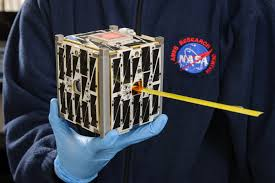
\includegraphics[scale=0.5]{figures/cubesat.jpg}
\caption{Referência de Tamanho de um Cubesat}
\label{figura_cubesat}
\end{center}
\end{figure}

Um dos novos desafios de desenvolvimento para \textit{Cubesats} é a limitação no orçamento, a qual torna necessária a realização de modelagens e simulações antes do desenvolvimento do produto, de forma a reduzir os custos. Outro desafio é a limitação na área disponível para captação e armazenamento de energia devido ao tamanho dos satélites\cite{Kalman2011}. Tendo em vista esta limitação no aspecto energético, é necessário projetar o sistema cuidadosamente de forma que a energia fornecida pelos painéis solares e armazenadas nas baterias seja suficiente para alimentar as cargas do sistema.

Os \textit{Cubesats} são, em geral, compostos por um Computador de Bordo, responsável por gerenciar os dados do satélite, um \gls{eps}, responsável por captar, armazenar e distribuir energia para os outros módulos, um Sistema de Comunicação, capaz de enviar e receber dados e comandos para a Terra e, por fim, os \textit{payloads}, que são a carga útil do sistema, ou seja, realizam a função principal do satélite.

Os \gls{eps} usam como principal entrada de energia painéis solares, que são a fonte mais abundante no espaço. Outra maneira de se captar energia é através de termogeradores. Para armazenar a energia são usadas geralmente bateris Li-Ion, porém alguns projetos utilizam supercapacitores ou baterias de composição diferente.

Neste trabalho será apresentado o \gls{eps} do \textit{Cubesat} FloripaSat, atualmente em desenvolvimento na UFSC, com foco no gerenciamento da energia, desde a entrada até o consumo dos outros módulos. Este \gls{eps} tem como entrada de energia painéis solares, que são conectados através de um conversor \textit{boost} a duas baterias Li-Ion conectadas em série. Um algortimo \gls{mppt} é utilizado para operar os paineis com máxima eficiência. O sistema distribui a energia para os outros módulos do satélite (computador de bordo, sistema de comunicação e \textit{payloads}) em diferentes tensões através de conversores CC-CC integrados. Um diagrama de blocos deste sistema pode ser visto na figura \ref{figura_diagrama_blocos}.

\begin{figure}[!htpb]
\begin{center}
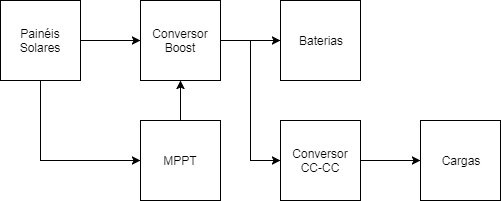
\includegraphics[scale=0.5]{figures/diagramaBlocos.png}
\end{center}
\caption{Diagrama de Blocos do Sistema}
\label{figura_diagrama_blocos}
\end{figure}


Será realizada a modelagem do sistema, simulações e, por fim, testes com o sistema real, de forma que será possível validar a simulação para trabalhos futuros assim como verificar se o sistema projetado está de acordo com o necessário.

\section{Objetivos}

Os objetivos gerais do trabalho são: modelar, simular e testar o funcionamento do módulo de energia do nanossatélite Floripa-Sat.

Como objetivos específicos podemos citar:
\begin{itemize}
\item Modelar os painéis solares
\item Modelar o conversor boost da entrada
\item Modelar o consumo do \textit{Cubesat}
\item Simular o sistema completo
\item Realizar testes com o sistema real
\item Comparar os resultados reais com os simulados
\end{itemize}

\section{Organização do trabalho}

O capítulo \ref{secao:painel solar} apresenta brevemente o funcionamento dos paineis solares, um circuito equivalente com componentes representando a conversão de energia solar em energia elétrica e as perdas, um modelo do painel real a ser utilizado no trabalho e por fim algoritmos para operação do painel com máxima eficiência.

No capítulo \ref{secao:conversores_cc_cc} são apresentadas duas maneiras de se utilizar conversores CC-CC no controle da operação de paineis solares e uma modelagem simplificada a ser utilizada na simulação do sistema.

O próximo passo é a modelagem das cargas do sistema (capítulo \ref{secao:modelagem_cargas}), para possibilitar a verificação do funcionamento do sistema na simulação. Para tal foram utilizadas informações fornecidas nos \textit{datasheets} dos principais componentes de cada módulo do satélite (comunicação, computador de bordo, sistema de energia e \textit{payloads}).

Nos capítulos \ref{secao:simulacao_sistema} e \ref{secao:teste_sistema}, respectivamente, são apresentados as simulações e testes realizados na bancada para verificar se o sistema projetado atende os requisitos de carga e também validar a simulação realizada em comparação com o sistema real.

Ao final do trabalho são apresentadas as conclusões sobre o que foi proposto e desenvolvido (capítulo \ref{secao:conclusoes}).



\printbibliography
\end{refsection}

\begin{refsection}
\chapter{Painel Solar}

O funcionamento de células solares é baseado no efeito fotovoltaico, ou seja, a geração de tensão ou corrente elétrica a partir da incidência de luz. O efeito fotovoltaico ocorre da seguinte maneira: em um semicondutor ideal existem dois níveis de energia que elétrons podem ser excitados, representados pela camada de valência, com energia baixa, e a camada de condução, com energia mais alta. Entre estas duas camada existe o chamado \textit{bandgap}, uma região de com níveis de energia que os elétrons não podem ter. Quando um fóton entra em contato com o semicondutor os elétrons na camada de valência absorvem sua energia e passam para a camada de condução, gerando uma corrente elétrica. Como não é possível que os elétrons possuam níveis intermediários de energia fótons que não possuam energia superior ao \textit{bandgap} não são absorvidos e passam sem interagir com a célula.\cite{jager2014}.

\section{Circuito Equivalente de um Painel Solar}

Em uma célula real existem perdas causadas por aquecimento no movimento dos elétrons, por impurezas no material que geram novos níveis de energia dentro do \textit{bandgap} e também por recombinação na junção p-n \cite{blakers2013}. Portanto para representar as células solares através de um circuito equivalente é necessário uma fonte de corrente associada com alguns componentes que representam as perdas.

O modelo para uma célula aqui utilizado é apresentado em \cite{erdem2013}. O circuito equivalente composto por uma fonte de corrente I\textsubscript{ph}, um diodo D, uma resistência paralela R\textsubscript{p} e uma resistência série R\textsubscript{s}. Este circuito pode ser encontrado na figura \ref{modelo_celula_solar}, onde I\textsubscript{ph} é a corrente fotogerada do painel, I\textsubscript{D} é a corrente do diodo, I\textsubscript{R\textsubscript{p}} é a corrente na resistência paralela, I é a corrente da célula e V é a tensão da célula.

\begin{figure}[!htpb]
\begin{center}
\begin{circuitikz} [american]
\draw
(0,0) to[I, l = I\textsubscript{ph}] (0,3) -- (2,3)
      to[diode, l = D] (2,0) -- (0,0)
(2,3) to[short] (4,3)
(4,3) to[resistor, l = R\textsubscript{p}] (4,0) -- (2,0)
(4,3) to [short] (4.5,3)
(4.5,3) to[resistor, l = R\textsubscript{s}] (6.5,3)
	  to[short, -o] (7,3)
(4,0) to[short, -o] (7,0)
(7,3) to[open, v=V] (7,0);
\draw[->] (6.25, 3.25) -- (7,3.25) node[midway, above] {I};
\draw[->] (2.25, 2.75) -- (2.25, 2) node[midway, right] {I\textsubscript{D}};
\draw[->] (4.25, 2.75) -- (4.25, 2) node[midway, right] {I\textsubscript{R\textsubscript{p}}};
\end{circuitikz}
\end{center}
\caption{Circuito equivalente da célula solar}
\label{modelo_celula_solar}
\end{figure}

A partir da análise do circuito equivalente, temos a seguinte relação entre a corrente e a tensão da celula:

\begin{equation} \label{eq:relacao_corrente_tensao_celula}
I = I_{ph} - I_{D} - I_{R_{p}}
\end{equation}

Por simplicidade e sem perda de precisão I\textsubscript{ph} pode ser determinada diretamente pela corrente de curto-circuito I\textsubscript{sc} do painel, respeitando-se a dependência com a irradiância E e a temperatura da célula T\textsubscript{c} (equação \ref{eq:corrente_fotogerada}), assim pode-se obtê-la diretamente dos \textit{datasheets} fornecidos pelos fabricantes. 

\begin{equation} \label{eq:corrente_fotogerada}
I_{ph} = I_{sc}\cdot \frac{E}{E_{0}} \cdot [1 + \Delta_{I_{sc}}(T_{c} - T_{0})]
\end{equation}

A corrente no diodo é dada pela equação \ref{eq:corrente_diodo}, onde I\textsubscript{o} é a corrente de saturação na sombra, q é a carga de um elétron, n é o fator de idealidade, k é a constante de Boltzmann e T\textsubscript{c} é a temperatura da célula \cite{bellia2014}.

\begin{equation} \label{eq:corrente_diodo}
I_{D} = I_{o}(e^{-\frac{q(V+I\cdot R_{s})}{nkT_{c}}}-1)
\end{equation}

A corrente no resistor R\textsubscript{p} pode ser obtida através da equação \ref{eq:corrente_Rp}, conhecida como lei de Ohm.

\begin{equation} \label{eq:corrente_Rp}
I_{R_{p}} = \frac{V+I\cdot R_{s}}{R_{p}}
\end{equation}

Combinando as equações apresentadas, obtem-se a equação \ref{eq:relacao_corrente_tensao_celula_com_parametros}, que mostra a relação entre a corrente e a tensão da celula solar a partir dos parâmetros do circuito equivalente.

\begin{equation} \label{eq:relacao_corrente_tensao_celula_com_parametros}
I = I_{ph} - I_{o}(e^{-\frac{q(V+I\cdot R_{s})}{nkT_{c}}}-1) - \frac{V+I\cdot R_{s}}{R_{p}}
\end{equation}

Quando várias células são conectadas em série e/ou em paralelo é formado um painel solar. As curvas características de corrente por tensão e potência por tensão de um painel podem ser vistas nas figuras \ref{figura_corrente_painel_temperatura} e \ref{figura_potencia_painel_temperatura}, onde é evidenciada a dependência com a temperatura e a irradiância. 

\pgfplotstableread[col sep = comma]{figures/solarPanelCharacteristics-25.csv}\solarPanelCharacteristicsMinusTwentyFive
\pgfplotstableread[col sep = comma]{figures/solarPanelCharacteristics0.csv}\solarPanelCharacteristicsZero
\pgfplotstableread[col sep = comma]{figures/solarPanelCharacteristics25.csv}\solarPanelCharacteristicsTwentyFive
\pgfplotstableread[col sep = comma]{figures/solarPanelCharacteristics50.csv}\solarPanelCharacteristicsFifty

\begin{figure}[!htpb]
\begin{minipage}{.5\textwidth}
\begin{center}
\begin{tikzpicture}[trim axis left, trim axis right]
\begin{axis}[xlabel = {V [\SI{}{\volt}]}, ylabel = {I [\SI{}{\ampere}]}, ymin = 0, yticklabel style={/pgf/number format/fixed}, xtick distance=1, legend pos = south west, scale = 0.5, scale only axis]
\addplot[mark = none, color = cyan] table[x index = {0}, y index = {1}]{\solarPanelCharacteristicsMinusTwentyFive};
\addplot[mark = none, color = blue, dotted] table[x index = {0}, y index = {1}]{\solarPanelCharacteristicsZero};
\addplot[mark = none, color = magenta, dashed] table[x index = {0}, y index = {1}]{\solarPanelCharacteristicsTwentyFive};
\addplot[mark = none, color = red, dash dot] table[x index = {0}, y index = {1}]{\solarPanelCharacteristicsFifty};
\addlegendentry{\SI{-25}{\celsius}}
\addlegendentry{\SI{0}{\celsius}}
\addlegendentry{\SI{25}{\celsius}}
\addlegendentry{\SI{50}{\celsius}}
\end{axis}
\end{tikzpicture}
\caption[caption]{Corrente de um painel \\\hspace{\textwidth} solar}
\label{figura_corrente_painel_temperatura}
\end{center}
\end{minipage}
\begin{minipage}{.5\textwidth}
\begin{center}
\begin{tikzpicture}[trim axis left, trim axis right]
\begin{axis}[xlabel = {V [\SI{}{\volt}]}, ylabel = {I [\SI{}{\watt}]}, ymin = 0, yticklabel style={/pgf/number format/fixed}, xtick distance=1, legend pos = north west, scale = 0.5, scale only axis]
\addplot[mark = none, color = cyan] table[x index = {0}, y index = {2}]{\solarPanelCharacteristicsMinusTwentyFive};
\addplot[mark = none, color = blue, dotted] table[x index = {0}, y index = {2}]{\solarPanelCharacteristicsZero};
\addplot[mark = none, color = magenta, dashed] table[x index = {0}, y index = {2}]{\solarPanelCharacteristicsTwentyFive};
\addplot[mark = none, color = red, dash dot] table[x index = {0}, y index = {2}]{\solarPanelCharacteristicsFifty};
\addlegendentry{\SI{-25}{\celsius}}
\addlegendentry{\SI{0}{\celsius}}
\addlegendentry{\SI{25}{\celsius}}
\addlegendentry{\SI{50}{\celsius}}
\end{axis}
\end{tikzpicture}
\caption[caption]{Potência de um painel \\\hspace{\textwidth} solar}
\label{figura_potencia_painel_temperatura}
\end{center}
\end{minipage}
\end{figure}

\pgfplotstableread[col sep = comma]{figures/solarPanelCharacteristics250.csv}\solarPanelCharacteristicsTwoHundredFifty
\pgfplotstableread[col sep = comma]{figures/solarPanelCharacteristics500.csv}\solarPanelCharacteristicsFiveHundred
\pgfplotstableread[col sep = comma]{figures/solarPanelCharacteristics750.csv}\solarPanelCharacteristicsSevenHundredFifty
\pgfplotstableread[col sep = comma]{figures/solarPanelCharacteristics1000.csv}\solarPanelCharacteristicsThousand

\begin{figure}[!htpb]
\begin{minipage}{.5\textwidth}
\begin{center}
\begin{tikzpicture}[trim axis left, trim axis right]
\begin{axis}[xlabel = {V [\SI{}{\volt}]}, ylabel = {I [\SI{}{\ampere}]}, ymin = 0, yticklabel style={/pgf/number format/fixed}, xtick distance=1, legend pos = south west, scale = 0.5, scale only axis]
\addplot[mark = none, color = cyan] table[x index = {0}, y index = {1}]{\solarPanelCharacteristicsTwoHundredFifty};
\addplot[mark = none, color = blue, dotted] table[x index = {0}, y index = {1}]{\solarPanelCharacteristicsFiveHundred};
\addplot[mark = none, color = magenta, dashed] table[x index = {0}, y index = {1}]{\solarPanelCharacteristicsSevenHundredFifty};
\addplot[mark = none, color = red, dash dot] table[x index = {0}, y index = {1}]{\solarPanelCharacteristicsThousand};
\addlegendentry{\SI[per-mode=symbol]{250}{\watt\per\meter\squared}}
\addlegendentry{\SI[per-mode=symbol]{500}{\watt\per\meter\squared}}
\addlegendentry{\SI[per-mode=symbol]{750}{\watt\per\meter\squared}}
\addlegendentry{\SI[per-mode=symbol]{1000}{\watt\per\meter\squared}}
\end{axis}
\end{tikzpicture}
\caption[caption]{Corrente de um painel \\\hspace{\textwidth} solar}
\label{figura_corrente_painel_irradiância}
\end{center}
\end{minipage}
\begin{minipage}{.5\textwidth}
\begin{center}
\begin{tikzpicture}[trim axis left, trim axis right]
\begin{axis}[xlabel = {V [\SI{}{\volt}]}, ylabel = {I [\SI{}{\watt}]}, ymin = 0, yticklabel style={/pgf/number format/fixed}, xtick distance=1, legend pos = south west, scale = 0.5, scale only axis]
\addplot[mark = none, color = cyan] table[x index = {0}, y index = {2}]{\solarPanelCharacteristicsTwoHundredFifty};
\addplot[mark = none, color = blue, dotted] table[x index = {0}, y index = {2}]{\solarPanelCharacteristicsFiveHundred};
\addplot[mark = none, color = magenta, dashed] table[x index = {0}, y index = {2}]{\solarPanelCharacteristicsSevenHundredFifty};
\addplot[mark = none, color = red, dash dot] table[x index = {0}, y index = {2}]{\solarPanelCharacteristicsThousand};
\addlegendentry{\SI[per-mode=symbol]{250}{\watt\per\meter\squared}}
\addlegendentry{\SI[per-mode=symbol]{500}{\watt\per\meter\squared}}
\addlegendentry{\SI[per-mode=symbol]{750}{\watt\per\meter\squared}}
\addlegendentry{\SI[per-mode=symbol]{1000}{\watt\per\meter\squared}}
\end{axis}
\end{tikzpicture}
\caption[caption]{Potência de um painel \\\hspace{\textwidth} solar}
\label{figura_potência_painel_irradiância}
\end{center}
\end{minipage}
\end{figure}

Como podemos ver pelas figuras, existe um ponto de máximo, conhecido como \gls{mpp}, e que este ponto varia muito com a variação da temperatura do painel e um pouco com a variação da irradiância incidente, portanto para operar o painel sempre com a maior eficiência é necessário aplicar uma técnica de controle conhecida como \gls{mppt} \cite{ahmed2016}.

\section{\glsentryshort{mppt}}

A impedância vista pelos terminais do painel determina o ponto de operação, de acordo com a equação \ref{eq:impedancia_painel}. Por conta deste fator, dificilmente um painel opera no \gls{mpp} quando conectado a uma carga arbitrária em um ambiente arbitrário. Para tal, são utilizados conversores CC-CC entre os painéis e a carga para realizar o casamento de impedância correto.

\begin{equation}
R = \frac{V}{I}
\label{eq:impedancia_painel}
\end{equation}

\subsection{Funcionamento dos Conversores CC-CC}

Para exemplificar o funcionamento dos conversores CC-CC em sistemas \gls{mppt} vamos considerar o caso de ser necessária tensão mais baixa na carga do que no painel, no qual é utilizado um conversor \textit{Buck}. O circuito deste sistema pode ser visto na figura \ref{circuito_com_conversor_buck}.

\begin{figure}[!htpb]
\begin{center}
\begin{circuitikz} [american]
\draw
(0,0) to[pvsource, l = V\textsubscript{pv}] (0,3)
      to[nos, l = S] (2,3)
(0,0) -- (2,0) to[diode, l = D]
(2,3) to[inductor, l = L] (4,3)
(4,3) to[capacitor, l = C] (4,0) -- (2,0)
(4,3) to[short] (6,3)
(6,3) to[resistor, l=R\textsubscript{L}] (6,0) -- (4,0)
(6,3) -- (8,3) to[open, v^=V\textsubscript{L}, o-o] (8,0) -- (6,0);
\draw[->] (-0.25, 2) -- (-0.25, 2.75) node[midway, left] {I\textsubscript{pv}};
\end{circuitikz}
\end{center}
\caption{Circuito com conversor \textit{Buck} para casamento de impedância}
\label{circuito_com_conversor_buck}
\end{figure}

As equações \ref{eq:ganho_estatico_conversor_buck} e \ref{eq:ganho_estatico_conversor_buck_corrente} representam o ganho estático de tensão e corrente do conversor \textit{Buck}.

\begin{equation} \label{eq:ganho_estatico_conversor_buck}
\frac{V_{L}}{V_{pv}} = D
\end{equation}

\begin{equation}\label{eq:ganho_estatico_conversor_buck_corrente}
\frac{I_{pv}}{I_{L}} = D
\end{equation}

Combinando estas duas equações na equação \ref{eq:relacao_impedancia_entrada_saida_buck} obtemos a relação entre a impedância de entrada e saída do conversor. Como a impedância de entrada é a impedância de saída do painel (carga do painel), podemos variar a razão cíclica D e consequentemente variar o ponto de operação do painel, de forma a sempre operar no ponto de máxima potência.

\begin{equation} \label{eq:relacao_impedancia_entrada_saida_buck}
\begin{aligned}
R &= \frac{V_{pv}}{I_{pv}} \\
&= \frac{V_{L}}{D} \cdot \frac{1}{I_{L}\cdot D} \\
&= \frac{1}{D^{2}} \cdot \frac{V_{L}}{I_{L}} \\
&= \frac{1}{D^{2}} \cdot R_{L}
\end{aligned}
\end{equation}

Outros exemplos de conversores CC-CC empregados em sistemas \gls{mppt} são os conversores \textit{Boost}, quando deseja-se uma tensão de saída maior que na entrada, e os conversores \textit{Buck-Boost}, que podem ser usados tanto para aumentar como para diminuir a tensão de saída em relação a tensão de entrada.

\subsection{Algoritmos}

\subsubsection{Perturba e Observa}



\printbibliography
\end{refsection}

\begin{refsection}
\chapter{Conversor Boost}
Para possibilitar o controle da tensão do painel solar e possibilitar a implementação do algoritmo MPPT foi utilizado um conversor boost. O circuito completo pode ser visto na figura \ref{circuito_completo}.

\begin{figure}[!htpb]
\begin{center}
\begin{circuitikz} [american]
\draw
(0,0) to[pvsource, l = V\textsubscript{pv}] (0,3)
      to[inductor, l = L] (2,3)
(2,3) to[nos, l = S] (2,0) -- (0,0)
(2,3) to[diode, l = D] (4,3)
(4,3) to[capacitor, l = C] (4,0) -- (2,0)
(5,2.025) node[nigfete, xscale=1, anchor=G, bodydiode, rotate=90] () {}
(6,2.025) node[nigfete, xscale=-1, anchor=G, bodydiode, rotate=90] () {}
(7,3) to[battery, v = V\textsubscript{bat}] (7,0) -- (4,0);

\draw[->] (-0.25, 2) -- (-0.25, 2.75) node[midway, left] {I\textsubscript{pv}};
\end{circuitikz}
\end{center}
\caption{Circuito completo}
\label{circuito_completo}
\end{figure}
\printbibliography
\end{refsection}

\begin{refsection}
\chapter{Modelagem das Cargas}

\section{Computador de Bordo}

O computador de bordo tem funções como armazenamento dos dados em memória não-volátil, leitura de sensores e aquisição dos dados dos demais módulos do satélite.

Alguns contribuintes para o consumo estão listados na tabela \ref{consumo_computador_bordo}. Como é possível observar, poucos componentes contribuem para a maior parte do consumo. O cálculo da potência consumida é realizado multiplicando a corrente consumida pela tensão de alimentação, de \SI{3.3}{\volt}, exceto em casos especiais onde a equação é fornecida pelo \textit{datasheet} do componente.

\begin{table}[!htpb]
\centering
\begin{tabular}{c c c c}
\\ \hline
Componente & Quantia & Corrente [\SI{}{\milli\ampere}] & Potência [\SI{}{\milli\watt}] \\ \hline \hline
\glsentryshort{imu} (MPU-9250) & 1 & 3.7 \cite{mpu9250} & 12.21 \\
\glsentryshort{imu} (BMX055) & 1 & 5.7 \cite{bmx055} & 18.81 \\
Gerador de Referência & 1 & 0.026 \cite{ref5030}, \cite{msp430f6659} & 0.0008 \cite{ref5030} \\
Amplificador Operacional & 4 & 0.2 \cite{tlv341} & 2.64 \\
\textit{Watchdog} Externo & 1 & 0.025 \cite{tps3823} & 0.0825 \\
microSD & 1 & 0.25 \cite{microSD} & 0.825 \\
Memória não-volátil & 3 & 0.05 \cite{is25lp128} & 0.495 \\
Microcontrolador & 1 & 8.39 \cite{msp430f6659} & 57.1134 \cite{msp430f6659} \\
Sensor de Corrente & 1 & 0.23 \cite{max9934} & 2.277 \\
Resistor Shunt (\SI{0.05}{\ohm}) & 1 & 19.271 & 0.01857 \\ \hline
Total & - & 19.271 & 94.47 \\ \hline
\end{tabular}
\caption{Consumo do Computador de Bordo}
\label{consumo_computador_bordo}
\end{table}

Aqui foram considerados apenas os consumos constantes, ou seja, o aumento no consumo durante comunicações do processador com outros dispositivos não foi considerado por apresentar um valor muito pequeno quando comparado com o constante (\SI{0.05}{\milli\watt} de média).

\section{Rádios e Amplificadores de Potência}

Os dois rádios do satélite têm como função enviar os dados coletados para a terra, através de telemetria. Durante a transmissão o consumo de potência é muito maior do em outros momentos, devido ao fato de que o \gls{pa} de cada rádio fica desativado. Portanto para modelar o consumo deste sistema será considerado apenas o comportamento dinâmico, de acordo com a tabela \ref{consumo_radios}. Como os dados enviados por cada rádio são diferentes, os períodos de transmissão e o tempo ativo também são diferentes.

\begin{table}[!htpb]
\centering
\begin{tabular}{c c c c}
\\ \hline
Componente & Período/ & Corrente [\SI{}{\ampere}] & Potência [\SI{}{\milli\watt}] \\
& Tempo Ativo [\SI{}{\second}] & & \\ \hline \hline
\glsentryshort{pa} (Transceiver) & 60/2 & 0.6 \cite{rf6886} & 1.98 \\
\glsentryshort{pa} (Beacon) & 10/0.6 & 0.6 \cite{rf6886} & 1.98 \\ \hline
Total & - & - & - \\ \hline
\end{tabular}
\caption{Consumo dos Rádios}
\label{consumo_radios}
\end{table}
\printbibliography
\end{refsection}

\end{document}
